\documentclass[oneside,a4paper,12pt]{article}
\usepackage{graphicx}
\usepackage[section]{placeins}
\usepackage{hyperref}
\graphicspath{{../images/}}

\makeindex
\begin{document}
	\begin{titlepage}
		
\includegraphics[width=4cm]{logopopo.png}
		\hspace*{\fill}
		
\includegraphics[width=6cm]{univlille.png}
		
		\begin{center}
			\vspace{1cm}
			\textbf{Etude de capteurs}\\
			\textbf{Le capteur de distance infra-rouge}\\
			\textbf{GP2D120}\\
			\vspace{1cm}
			\textbf{Valentin DOSIAS, Konstantin PATRIKEV,}\\
			\textbf{Lennyn YUICHI, Maxence NEUS}\\
			\vspace{3cm}
			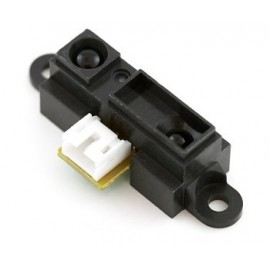
\includegraphics[width=8cm]{capteur.jpg}\\
			\vspace{\fill}
			\textbf{Octobre 2021}\\
		\end{center}
	\end{titlepage}

	\tableofcontents
	\newpage
	
	\section{Présentation du capteur\\ -- Lennyn YUICHI}
	\paragraph{}
	Les robots mobiles autonomes sont des machines capables de se déplacer dans leur environnement, sans interférence humaine directe. Malgré le grand potentiel de ces robots, ils sont encore peu utilisés dans l'industrie, comme c'est le cas pour les robots fixes. L'une des raisons en est la grande complexité des systèmes de commande de robots mobiles. Cependant, la recherche en robotique mobile laisse présager un avenir très différent, car les robots mobiles sont bien plus polyvalents que les robots fixes.
	\paragraph{}
	Il existe deux approches de base pour contrôler les robots mobiles : délibérative et réactive. Alors que l'approche délibérative utilise la planification pour décider du meilleur comportement pour le robot, l'approche réactive crée simplement une association directe entre les données reçues des capteurs et les actions à effectuer par le robot. De plus, comme la planification nécessite une connaissance préalable de l'environnement du robot, l'approche réactive est plus appropriée lorsque le robot doit explorer un environnement totalement inconnu.\\
	\paragraph{}
	En général, chaque système autonome utilise, de manière basique, des capteurs, des actionneurs et des processeurs pour effectuer avec succès une certaine tâche. C'est à travers l'étape de détection qu'il est possible de surveiller un certain processus.\\
	Les capteurs sont, en gros, des appareils qui effectuent la mesure d'une certaine quantité physique, le résultat de cette mesure est converti en signaux de tension électrique, afin que le processeur en question puisse acquérir ces données.\\
	Il existe essentiellement deux classes de capteurs : analogiques et numériques. Les capteurs analogiques sont ceux qui ont des valeurs de tension différentes dans une certaine plage à leur sortie. Les capteurs numériques, d'autre part, présentent des signaux binaires dans leur sortie. Robotino 2, par exemple, est équipé de deux capteurs analogiques (capteur de distance infrarouge et capteur inductif) et d'un capteur numérique (capteur optique).\\
	
	\paragraph{}
	L'objet d'étude de ce rapport était l'un des 3 types de capteurs présents dans Robotino 2: Le capteur de distance infrarouge (GP2D120). Ce robot est équipé de 9 de ce capteur, chacun espacé d'un angle de 40°, afin de couvrir toute la région qui l'entoure. N'oubliez pas qu'il est possible de manipuler chacun de ces capteurs individuellement, via la carte d'E/S.
	\paragraph{}
	De manière générale, les capteurs infrarouges sont utilisés pour déterminer la distance à un objet particulier. Ce type de capteur est répandu dans les domaines les plus divers, notamment dans les applications autonomes. En robotique, par exemple, ces capteurs peuvent être utilisés pour éviter les collisions, pour positionner le robot ou même pour effectuer une tâche.
	\paragraph{}
	Les capteurs de distance infrarouges se composent d'un émetteur et d'un récepteur. L'émetteur envoie un rayon infrarouge, dont la réflexion est captée par le récepteur et convertie en une valeur de tension inversement proportionnelle à la distance entre le robot et l'objet. La figure 1 présente un graphique de la distance par rapport à la tension du capteur GP2D120.
	\begin{figure}[h]
		\centering
		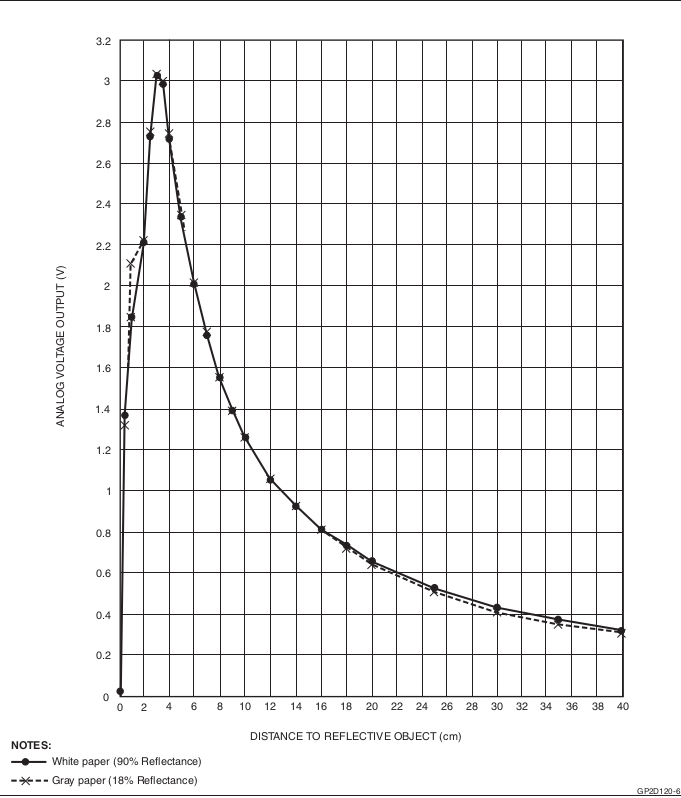
\includegraphics[width=8cm]{screenDatasheet.png}
		\caption{Caractèristique présentée dans la datasheet}
	\end{figure} 
	\paragraph{}
	Comme le montre le graphique de la figure 1, le capteur GP2D120 est un capteur analogique, c'est-à-dire qu'il présente, dans sa sortie, des valeurs comprises dans une certaine plage. Il est à noter que ce capteur effectue des mesures précises à des distances de 4 cm à 30 cm, ainsi, il est possible d'obtenir à partir du graphique de la figure 1, les valeurs typiques maximale et minimale de la tension de sortie de ce capteur. La figure 2 présente les caractéristiques techniques de fonctionnement de ce capteur.\\
	
	\begin{figure}[h]
		\centering
		\caption{Caractéristiques techniques du capteur GP2D120}
		\begin{tabular}{|p{0.18\textwidth}|c|p{0.16\textwidth}|c|c|c|c|}
			\hline
			Paramètre & Symbole & Condition & Minimum & Typique & Maximum & Unité \\
			\hline
			Plage de distance de mesure & $\Delta L$ & & 4 & - & 30 & cm \\
			\hline
			Tension aux bornes de sortie & Vo & L = 30 cm & 0,25 & 0,4 & 0,55 & V \\
			\hline
			Différence de tension de sortie & $\Delta Vo$ & Changement de sortie à
			$\Delta L$ (30 - 4) cm & 1,95 & 2,25 & 2,55 & V \\
			\hline
			Courant d'alimentation moyen & Icc & L = 30 cm & - & 33 & 50 & mA \\
			\hline
			Tension d'alimentation & Vcc &  & 4,55 & 5,0 & 5,55 & V \\
			\hline
			
			
		\end{tabular}
	\end{figure}

	\paragraph{}
	En ce qui concerne les erreurs de mesure, comme tout autre capteur, les capteurs de distance infrarouges sont sujets à des imprécisions lors des mesures, cependant, il existe des moyens de minimiser ces erreurs. Il est possible, par exemple, de rendre la mesure plus efficace en changeant la position du capteur (verticale ou horizontale). Si la surface réfléchissante a deux matériaux/couleurs différentes, il est recommandé de positionner le capteur de manière à ce qu'il soit parallèle à la ligne de démarcation entre ce matériau/couleur, afin de minimiser les erreurs de mesure.\\
	Une autre façon de minimiser ces erreurs concerne les facteurs d'éclairage externes. Dans certains cas, il est possible que le capteur ne mesure pas correctement s'il est directement exposé à la lumière. Il convient de rappeler qu'il existe plusieurs autres moyens d'éviter les erreurs de mesure, en fonction de l'application du capteur.
	
	
	\newpage
	
	\section{Principe de fonctionnement\\ -- Konstantin PATRIKEV}
	\paragraph{}
	Nous allons dans cette partie définir le principe de fonctionnement de ce capteur en passant par l'explication des lois physiques et mathématiques qui déterminent le système.\\
	
	\subsection{Principe de fonctionnement global}
	\paragraph{}
	Le principe de ce capteur par réflexion est d'éclairer l’obstacle avec une led infrarouge, et de mesurer la quantité de lumière réfléchie par la surface avec une photodiode PSD (Position Sensitive Detector).
	\paragraph{}
	La photodiode est un photodétecteur qui fonctionne par absorption de photons infrarouge. L’objet éclairé transmet une énergie inversement proportionnelle au carré de la distance. On peut voir le schéma bloc du système étudié ci dessous:
	
	\begin{figure}[h]
		\centering
		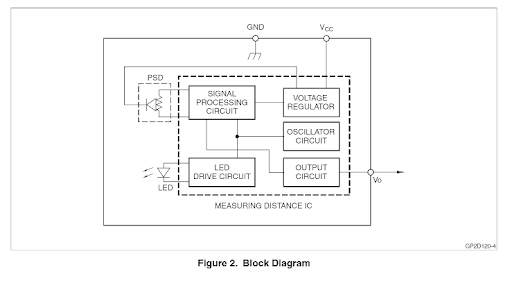
\includegraphics[width=10cm]{img3.png}
		\caption{Block diagram}
	\end{figure} 
	\paragraph{}
	On peut notamment y voir une photodiode PSD qui sert de récepteur et une LED infrarouge émettant à une longueur d’onde  $\lambda$ = 850 nm avec une précision de 50 nm (donnés constructeur). 
	\paragraph{}
	Une photodiode (semi-conducteur polarisé en inverse) laisse passer un courant inversement proportionnel à l’énergie lumineuse reçue et possède un courant de fuite (courant émis dans l’obscurité).\\
	La distance capteur-émetteur sera mesurée en volts et transmise en Vo par le processeur de signal numérique (signal processing circuit).
	\subsection{Principe de réflexion d’une onde}
	\paragraph{}
	La réflexion est définie comme le changement de direction d’une onde à la rencontre de 2 milieux, donc entre l’air et la surface blanche du mur dans notre cas. Après réflexion, au niveau de l’interface entre les 2 milieux, on a l’apparition d’une onde réfléchie, qui servira à calculer la distance, et d’une onde transmise.\\
	
	Notons que le rayonnement à détecter correspond à une énergie $ E= \frac{hc}{\lambda} \ = 2.34 E-19 J = 1.24 eV $  (avec h la constante de Planck et c la vitesse de la lumière).
	
	\subsection{Principe de triangulation}
	
	\begin{figure}[h]
		\centering
		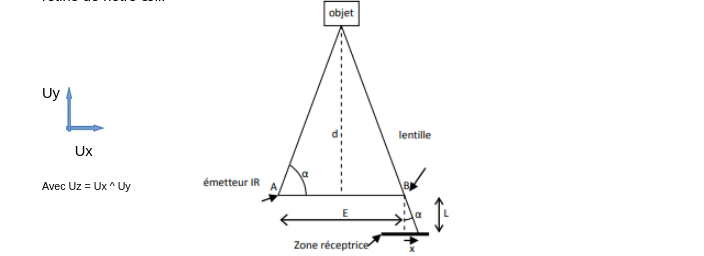
\includegraphics[width=12cm]{img4.png}
		\caption{Schéma du parcours de l’onde entre l'émetteur IR et la zone réceptrice du capteur}
	\end{figure} 

	\begin{itemize}
		\item[$\alpha$] angle de réflexion (rad)
		\item[x] position de l’onde réfléchie sur le récepteur (m)
		\item[L] distance entre le récepteur et l'émetteur sur le vecteur unitaire Uy (m)
		\item[d] distance mesurée (m)
		\item[x] distance entre le récepteur et l'émetteur sur le vecteur unitaire  Ux (m)
	\end{itemize}

	D’après les lois trigonométriques, on peut affirmer que:\\
	$$ tg . \alpha = \frac{2d}{E} = \frac{x}{L} (tg = angle\ oppos\acute{e}/angle\ adjacent)$$ 
	$$ D’o\grave{u}\ d = \frac{E}{2L}x \ \  avec\ E\ et\ L\ connus. $$
	
	Comme dit précédemment, la zone réceptrice et un PSD: Il est composé de 2 diodes PIN avec leur cathode commune. Ce capteur renvoie la position moyenne du barycentre de la zone illuminée car l'émetteur IR possède un cône d’émission assez large comme vu sur le schéma ci-dessous qui montre en détail la composition de la partie réceptrice du capteur:\\

	\begin{figure}[h]
		\centering
		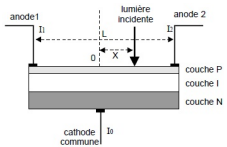
\includegraphics[width=10cm]{img5.png}
	\end{figure} 
	
	Un barycentre correspond à la position de la lumière incidente sur la zone réceptrice dans le plan (Ux,Uz).\\
	
	
	\section{Modélisation de la caractèristique du capteur\\ -- Maxence NEUS}
	
	\paragraph{}
	Le modele de capteur qui est utilisé sur le Robotino est le GP2D120 de chez Sharp, le constructeur fourni dans la datasheet plusieurs informations. Nous allons ici nous interesser plus particulièrement à la caractèristique entrée-sortie du capteur, c'est à dire la relation :
	\begin{center}
		${Tension\ de\ sortie = f(Distance)}$
	\end{center}
	La connaissance de cette caractèristique est trés importante pour l'utilisation du capteur, en effet sans connaître la relation qui lie la tension lue à la distance aui a été mesurée, la sortie du capteur est complètement inutilisable.\\
	
	La datasheet du capteur propose la caractèristique en tension en figure 1. Grace à celle-ci, on peut en apprendre plus sur notre capteur.\\
	Ignorons dans un premier temps le début de la courbe jusqu'à environ 4cm.\\
	\paragraph{}
	Tout d'abord, pour ce qui est de la préçision du capteur:\\
	On voit que lorsque la distance est proche des 4cm, la pente de la courbe est trés prononçée, ce qui fait que de faibles différences dans la distance se font grandement ressentir sur la tension à la sortie.\\
	\`{A} contrario, lorsque la distance augmente, la pente de la courbe diminue grandement elle aussi, pénalisant alors la préçision sur cette plage de distances.\\
	Revenons maintenant sur la partie de la courbe qui correspond aux trés faibles distances. On observe ici un phénomène inhérent au principe de fonctionnement du capteur, en effet il existe une distance limite à partir laquelle le capteur est trop proche de l'objet pour réaliser une mesure correcte.
	
	
	\begin{figure}[h]
		\centering
		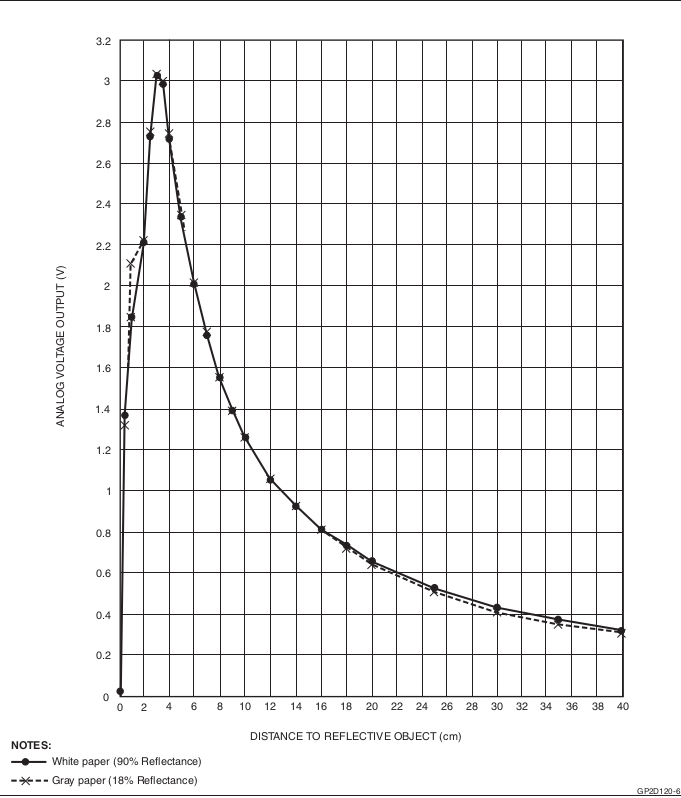
\includegraphics[width=8cm]{screenDatasheet.png}
		\caption{Caractèristique présentée dans la datasheet}
	\end{figure} 

	
	\begin{figure}[h]
		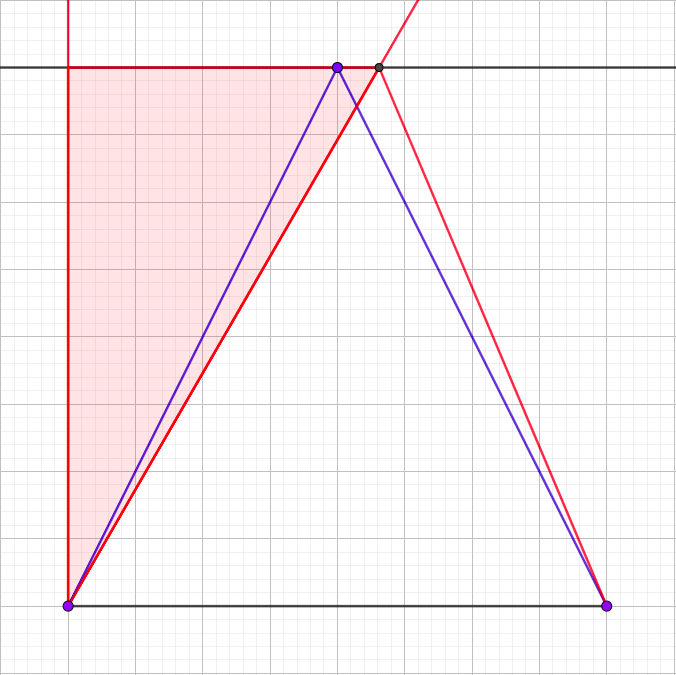
\includegraphics[width=5cm]{goodCase.png}
		\hspace*{\fill}
		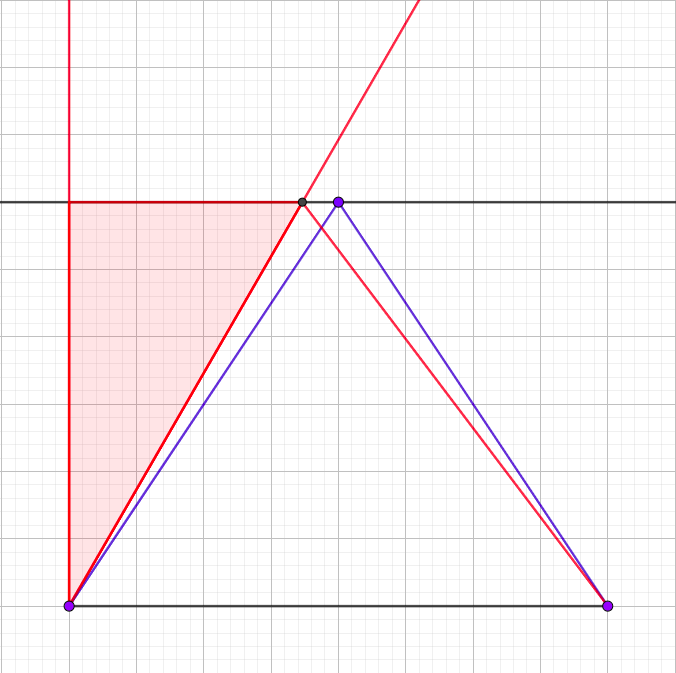
\includegraphics[width=5cm]{badCase.png}
		\caption{Illustration de l'erreur de mesure pour des petites distances}
	\end{figure}
	
	\paragraph{}
	Sur les graphs de la figure 6, le chemin bleu représente le chemin qui est supposé avoir été pris lors du calcul de la distance. Il est facile à voir aue celui-ci est toujours plus court que le chemin rouge, ce qui fait que dans le cas o\`{u} la distance est suffisament grande, c'est la lumière qui a emprunter ce chemin qui arrive en premier au capteur. Dans le cas non favorable o\`{u} la distance est trop faible, le chemin rouge est le seul qui permet à la lumière d'arriver au capteur. Comme celui-ci est plus long, le capteur mesure une distance plus grande, ce qui se traduit par une tension plus faible sur la \\caractèristique.\\
	
	\newpage
	
	
	\newpage
	\section{Validation du modele\\ -- Valentin DOSIAS}
	\paragraph{}
	Sur le logiciel, les capteurs nous renvoient en pratique une tension comprise entre 0.3 et 2.54 Volts. Pour contrôler la fiabilité des capteurs, nous avons d’abord testé un seul capteur pour étudier la tension renvoyée en fonction de la distance. Sur le modèle de Robotino étudié, nous avions la distance affichée à l’écran. Nous nous sommes assurés que celle-ci soit correcte en réalité. Avec le capteur numéro 1, nous avons relevé la distance affichée à l’écran et la tension affichée sur le logiciel. Notre obstacle était un mur blanc de l’espace déstiné au Robotino dans la salle C305.\\
	\paragraph{}
	Sur nos premiers relevés nous avons d’abord remarqué que le capteur était efficace entre 4 cm et 40 cm environ. A 4 cm le capteur semblait avoir atteint un maximum de 2.54 Volts en dessous de cette distance, les valeurs de la tension commençaient à chuter et variaient constamment . Nous avons donc choisi de ne pas mesurer les différentes valeurs entre 0 et  4 cm.  Au delà d'environ 40 cm, les valeurs de tensions ne variaient que très peu et les valeurs de distance commençaient à être erronées comparé à la réalité. Nos premières remarques sont en accord avec la datasheet qui nous présente ce capteur comme efficace entre 4 et 30 cm.
	Nous avons obtenu la caractéristique suivante : \\
	
	\begin{figure}[h]
		\centering
		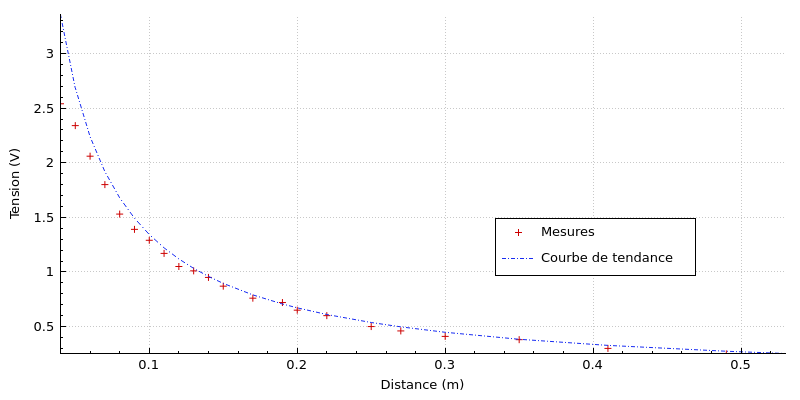
\includegraphics[width=12cm]{mesures.png}
		\caption{Tension déliverée par le capteur en fonction de la distance}
	\end{figure}
	\newpage
	La forme de la courbe est très semblable à celle de la datasheet. 
	
	En relevant les points de la datasheet, nous n’avons pas directement les valeurs précises mais nous pouvons les déduire approximativement à l’aide du graphique.
	
	
	\begin{figure}[h]
		\centering
		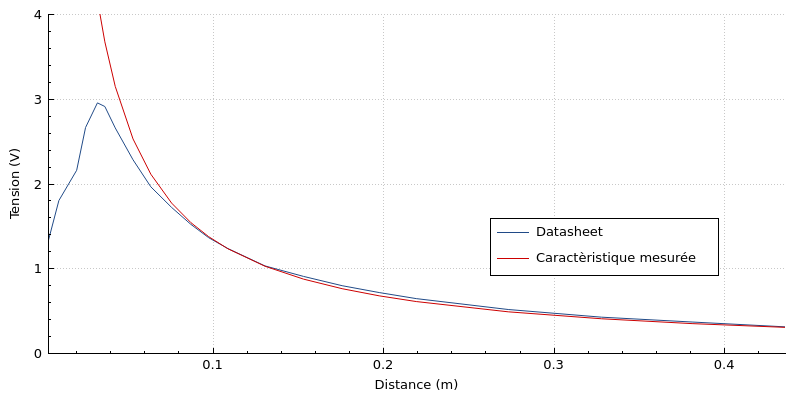
\includegraphics[width=12cm]{Comparedatasheet_mesures_v-d2.png}
		\caption{Comparaison des relevés avec la caractèristique de la datasheet}
	\end{figure}
	
	Ainsi en rentrant certaines données de l’expérience et les données relevées avec la datasheet. Nous voyons que les valeurs sont très proches, les deux courbes de tendance sont quasiment superposées.
	Pour les valeurs où nous avons les données de la datasheet et des relevés, nous pouvons calculer l’écart. Cela nous donne le résultat suivant.
	
	\begin{figure}[h]
		\centering
		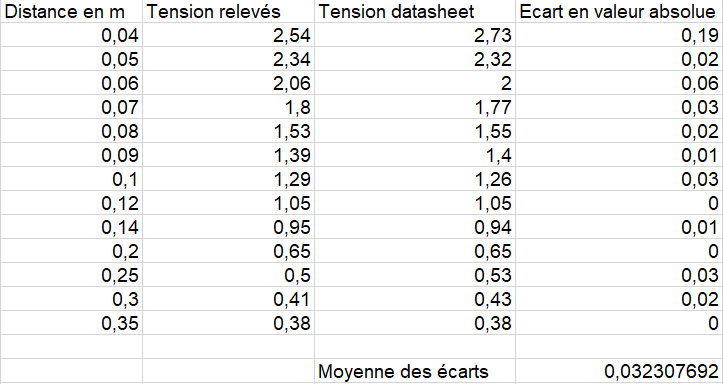
\includegraphics[width=12cm]{tab1.png}
	\end{figure}

	\paragraph{}
	Ainsi nous avons une valeur maximale d’écart de 0.19 V, mais cette valeur est à 4cm soit la limite de fonctionnement du capteur. La moyenne des écarts est de 0.03 V. Cette valeur est assez faible. Le capteur du Robotino est donc bien en accord avec son fonctionnement théorique.\\
	Nous allons maintenant nous intéresser à la différence de fonctionnements entre tous les capteurs. Pour ce faire nous avons relevé les différentes valeurs pour les capteurs à une certaine distance. Cette distance était de 20 cm quel que soit le capteur. Nous avons donc relevé les distances affichées sur l’écran du Robotino et la valeur de la tension affichée par le logiciel. La valeur théorique de la tension est calculée avec la formule de la courbe de tendance des données de la datasheet.
	
	\begin{figure}[h]
		\centering
		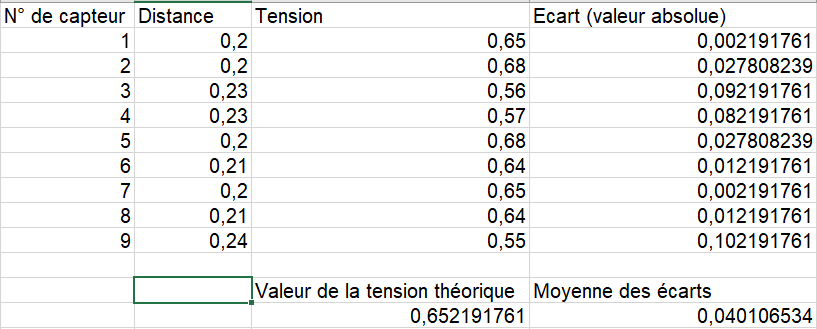
\includegraphics[width=12cm]{tab2.png}
	\end{figure}
	
	\paragraph{}
	Nous observons une erreur maximum de 4 cm provoquée à cause d’un écart de tension de 0,1 Volt par rapport à la valeur théorique. Cela représente une erreur d'environ 20\% pour le capteur le plus défectueux. Cet écart est assez important, il peut être dérangeant selon les utilisations du robot mais par exemple pour de la détection d’obstacle cet écart ne pose pas de problème. En moyenne, nous avons un écart de 6\% avec la valeur théorique ce qui est plutôt faible.
	\paragraph{}
	Ainsi, les caractéristiques théoriques du capteur sont en majorité bien respectées en réalité. Pour les capteurs ayant une distance de 21 cm, il est possible que nous ayons légèrement bougé le robot pendant la manipulation. De plus, les valeurs de la tension étaient instable à l’écran, nous devions arbitrairement choisir une valeur pour nos relevés ce qui peut causer une légère erreur de l’ordre de la moyenne des écarts.\\
	
	
	\section{Etude de marché\\ -- Valentin DOSIAS}
	\paragraph{}
	Tout d’abord pour l’étude de marché, il faut avoir conscience que ce capteur est assez vieux et aujourd’hui difficile à acheter. La première datasheet que nous avons trouvé de ce capteur datait de 1999 et celle que nous avons utilisé pour les parties précédentes datait de 2006.\\
	Le capteur est aujourd’hui affiché à 20€ mais apparaît en rupture de stock sur les plusieurs sites que nous avons consulté. Nous sommes plutôt redirigé vers ce qui semble être une version différente du capteur. 
	Le GP2YOA21YK0F est aussi un capteur de mesure de distance de la marque SHARP. Selon les résultats sur les sites de recherche, il semble plus populaire.\\
	\begin{figure}[h]
		\centering
		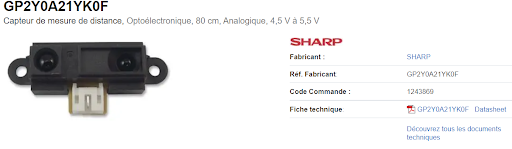
\includegraphics[width=12cm]{img1.png}
	\end{figure}
	\begin{figure}[h]
		\centering
		\caption{Comparaison des deux capteurs}
		\begin{tabular}{|p{0.33\textwidth}|c|c|}
			\hline
			Caractéristiques & GP2YOA21YK0F & GP2D120 \\
			\hline
			Caractéristiques & GP2YOA21YK0F & GP2D120 \\
			\hline
			Prix & ~12-13€ & ~20€ \\
			\hline
			$V_{in}$ (V) & 4.5-5.5 & 4.5-5.5 \\
			\hline
			$V_{out}$ (V) & 0-3.2 & 0-3 \\
			\hline
			Plage de distance (cm) & 10-80 & 4-30 \\
			\hline
			Consommation de courant (mA) & 30 & 33 \\
			\hline
		\end{tabular}
	\end{figure}
	\paragraph{}
	En effet, ce capteur semble plus populaire selon les résultats de recherches en tapant la référence du capteur du robotino nous tombons essentiellement sur le capteur présenté précédemment. Nous pouvons donc nous questionner sur le choix du capteur par les concepteurs. Il est possible que le capteur soit plus précis sur sa zone de détection. Par exemple, dans la majorité des cas 20 cm sera strictement 20cm pour le GP2D120 alors que pour le deuxième la distance affichée sera peut-être de 25 cm au lieu de 20 cm.\\
	Dans le cadre du Robotino, en mélangeant les différentes possibilités d'utilisations et les différents capteurs, les concepteurs ont sûrement jugé que cette distance devait être optimale.\\
	Une version plus disponible du capteur donc peut-être plus récente est le GP2Y0A41SK0F, il présente les mêmes caractéristiques, le même schéma bloc. et est affiché au prix de 10-11 € environ. Seul son temps de réponse semble meilleur, nous passons de 39ms à 16,7ms.
	
	\paragraph{}
	
	Nous allons maintenant nous intéresser aux capteurs d’autres marques. 
	Lorsque nous recherchons d’autres produits utilisant d’autres technologies, la marque SHARP semble être les leaders dans ce domaine avec des produits de différentes gammes (4-30cm et 10-80cm), les autres produits s’utilisent différemment ou utilisent une technologie différente.\\
	Nous avons notamment le capteur VCNL3040 de chez Vishay, transmettant son information de sortie non pas avec une tension mais avec un bus I2C. Il est vendu aux prix de 2.60€. La tension d’alimentation est de 2.5V à 3.6 V et la distance maximale de détection selon la datasheet est de 30cm, la distance minimale n’est pas précisée. De plus, sur la datasheet nous n’avons pas les mêmes courbes et informations que les capteurs de chez Sharp ce qui peut être un inconvénient pour les concepteurs. Les imprécisions de mesure ne peuvent pas être jugées de la même manière et leur intégration dans le système est très différente.\\
	\newpage
	\begin{figure}[h]
		\centering
		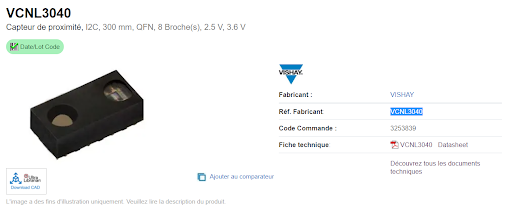
\includegraphics[width=12cm]{img2.png}
	\end{figure}
	\paragraph{}
	D’autres capteurs, dans la même gamme de prix existent mais utilisent des rayons infrarouges. Ils ont une plage de distance plus importante. Par exemple, le GP2Y0A41SK0F de chez sharp a une distance de détection couverte de 4 à 55 cm. 
	\paragraph{}
	Ainsi, nous avons une grande difficulté pour trouver des capteurs similaires et dans la même gamme de distance chez d’autres marques. Tous possèdent des attributs différents que ce soit la communication entre le capteur et le système ou la technologie utilisée. La plupart des autres capteurs utilisent des bus I2C et non pas une tension analogique de sortie.
	
	\newpage
	\section{Conclusion\\ -- Maxence NEUS}
	\paragraph{}
	Pour finir sur l'étude de ce capteur de distance à infra-rouge, bien que sa caractèristique nous montre qu'il n'est réellement utilisable que sur de courtes distances son utilisation dans le cadre du fonctionnement du Robotino a du sens dans la mesure o\`{u} il n'est utilisé que pour détecter la présence d'obstacles. En effet il n'est important de connaître la distance précise à laquelle se trouve l'obstacle que lorsque celui-ci est assez proche pour risquer une collision avec le robot.\\
	De plus, le comportement problématique du capteur pour les trés faibles distances ne pose ici pas de soucis majeurs de par la présence des bumpers qui allertent le robot des obstacles en collision.
	\paragraph{}
	Par ailleur la taille relativement petite du capteur ainsi que sa faible consommation en énergie nous permet d'en disposer un grand nombre sur tout le périmetre du robot ce qui apporte une vision trés utile pour son contrôle.\\
	
	\newpage
	\section{Sources}
	\url{http://fltsi.fr/tsi/tsi1/projet/Chaine\%20d\%27information/acquerir/capteur\%20infrarouge/capteurs\_IR.pdf}\\
	
	\url{https://fr.farnell.com/search?st=capteur%20de%20distance%20opto%C3%A9l%C3%A9ctronique}\\
	
	\url{https://www.conrad.fr/p/sharp-gp2d120-1-pcs-185336}\\
	
	\url{https://www.mouser.fr/c/?q=proximity%20optoelectronic%20sensor&OrgTerm=capteur%20opto%C3%A9l%C3%A9ctronique%20proximit%C3%A9&NewSearch=1}\\
	
	\url{https://www.farnell.com/datasheets/2856448.pdf}\\
	
	\url{https://www.festo-didactic.com/int-en/services/printed-media/technical-documentation/robotino-manual-544305.htm?fbid=aW50LmVuLjU1Ny4xNy4zMi45MDguNjcwOA}\\
	
	\url{https://www.pololu.com/file/0J157/GP2D120-DATA-SHEET.pdf}
	
	
	
	
\end{document}